\section{Theoretical framework}
\label{sec:theory}
\paragraph{}In order to be convenient for the future combination in different Higgs decay channel, the basic theory considered in this analysis keeps consistency with previous Higgs CP test in di-tau channel. The effective Lagrangian is the SM Lagrangian augmented with CP-odd operator of mass dimension 6, involving the Higgs field and electroweak gauge field. The other interaction between Higgs/vector boson and fermions/gluons is assumed to be the same with SM prediction. The Lagrangian could be written as: 

\begin{center}
\begin{math}
\mathcal{L}_{eff} = \mathcal{L}_{SM}+ \tilde{g}_{HAA}H\tilde{A}_{\mu\nu}A^{\mu\nu} + \tilde{g}_{HAZ}H\tilde{A}_{\mu\nu}Z^{\mu\nu} + \tilde{g}_{HZZ}H\tilde{Z}_{\mu\nu}Z^{\mu\nu} + \tilde{g}_{HWW}H\tilde{W}_{\mu\nu}^{+}W^{-\mu\nu}
\end{math}
\end{center}

Where $V^{\mu\nu}$ and $\tilde{V}^{\mu\nu}=\epsilon^{\mu\nu\rho\sigma}V_{\rho\sigma} $ (with $V=W^{\pm},Z,A$) denotes the vector field strength. Among the 4 coupling constants $g_{HVV}$ only 2 of them are independent due to the U(1)*SU(2) constrain, they can be written into 2 dimensionless coupling $\tilde{d}$ and $\tilde{d}_B$. As the different contribution from various vector electroweak gauge boson fusion process could not be distinguished experimentally, an arbitrary choice $\tilde{d}$ = $\tilde{d}_B$ is adopt. So the following relation could be derived: 

\begin{center}
\begin{math}
\tilde{g}_{HAA} = \tilde{g}_{HZZ} = \frac{1}{2} \tilde{g}_{HWW} = \frac{g}{2m_{W}}\tilde{d} \qquad and \qquad \tilde{g}_{HAZ}=0
\end{math}
\end{center}

The parameter $\tilde{d}$ becomes the only one describing the CP violation in VBF Higgs production. The corresponding matrix element could be written as the sum of a CP-even SM contribution $\mathcal{M}_{SM}$ and a CP-odd contribution $\mathcal{M}_{CP-odd}$ from EFT, and $\tilde{d}$ could be factorized out:

\begin{center}
\begin{math}
\mathcal{M}=\mathcal{M}_{SM}+\tilde{d}\cdot\mathcal{M}_{CP-odd} 
\end{math}
\end{center}

The VBF cross section is proportional to the squared matrix element: 

\begin{center}
\begin{math}
|\mathcal{M}|^2 = |\mathcal{M}_{SM}|^2 + \tilde{d}\cdot2 Re(\mathcal{M}^{\ast}_{SM} \mathcal{M}_{CP-odd}) + \tilde{d}^2\cdot|\mathcal{M}_{CP-odd}|^2
\end{math}
\end{center}

The first term and last term are both CP-even, only the second term from the interference of 2 matrix element is CP-odd, representing a new source of CPV in Higgs field. This CP-odd term would vanish after integrated after a CP-symmetric phase space, so it does not contribute to the total cross section and observed event yields after applying CP-symmetric selection criteria. The third term could increase the total cross section by an amount of $\tilde{d}^2$. 

\begin{comment}
\paragraph{}In the decay mode the EFT operator brings new source for Higgs decay to di-photon final state. At tree level these effective operators will contribute to the partial decay width of Higgs boson in $H\to\gam\gam$, $H\to\gam Z$, $H\to ZZ$ and $H\to WW$ channels. The helicity configuration of the particles in the final state is orthogonal to the SM case, so the interference term is zero. The angular distribution for the final state photon would not be influenced so only the change in number of branching ratio is considered: 

\begin{equation}
\label{eq:Bryy}
\small
\begin{aligned}
Br(H\to\gam\gam) &= \frac{\Gamma(H\to\gam\gam)_{SM}+\delta\Gamma(H\to\gam\gam)}{\Gamma(H)_{SM}+\delta\Gamma(H\to\gam\gam)+\delta\Gamma(H\to\gam Z) + \delta\Gamma(H\to Z^{\ast}Z) + \delta\Gamma(H\to W^{\ast}W)} \\
 & = \frac{0.227\% \times 4.066MeV + 155.425MeV \tilde{g}_{HAA}^2} { 4.088MeV+155.425MeV \tilde{g}_{HAA}^2+7.957MeV \tilde{g}_{HAZ}^2 + 0.00065MeV \tilde{g}_{HZZ}^2 + 0.0036MeV \tilde{g}_{HWW}^2 } 
\end{aligned}
\end{equation}

The numerical contribution from the branching ratio is significant compared with the SM prediction, only using the event yield can already provide a strict constraint on the CPV in this model. However, considering the cross section could be influenced by other CP-conserving new physics, event yields are unconstrained in the main part of this analysis.

\begin{figure}[h]
   \centering
   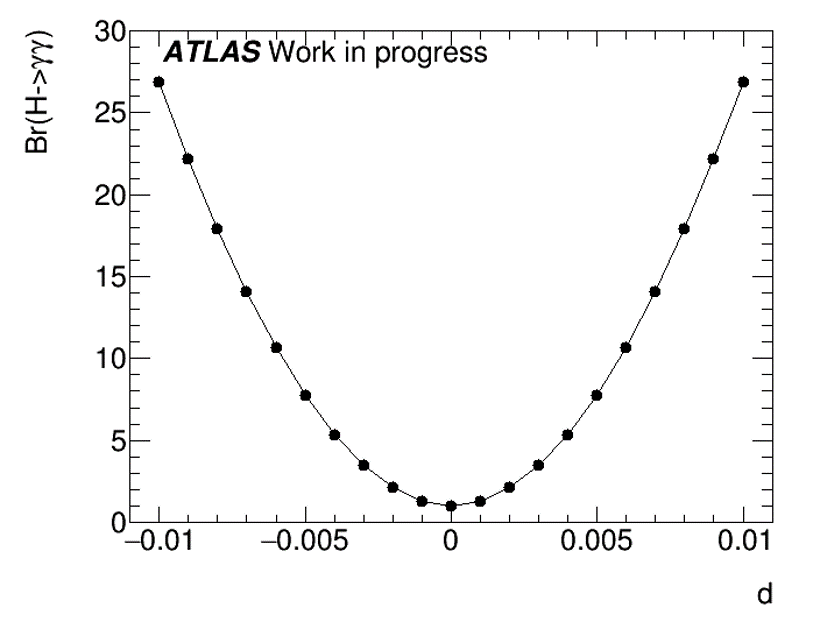
\includegraphics[width=.7\textwidth]{figure/BrHyy.png}
   \caption{Higgs to di-photon branching ratio as a function of CP mixing parameter $\tilde{d}$. }
   \label{fig:BrHyy}
\end{figure}
\end{comment}

\paragraph{}The VBF Higgs decay final state contains the reconstructed Higgs boson and two tagging jets from VBF topology. This can be characterized in a seven-dimension phase space, when fixing the Higgs mass, neglecting jet masses and exploiting the transverse momentum conservation. The Optimal Observable combines the information from total phase space into one single variable, so it shows much better performance than traditional operators. It is defined as the ratio of the interface term in the matrix element to the SM contribution: 

\begin{center}
\begin{math}
\mathcal{OO} = \frac{2Re(\mathcal{M}^{\ast}_{SM} \mathcal{M}_{CP-odd})}{|\mathcal{M}_{SM}|^2}
\end{math}
\end{center}


\paragraph{}The Optimal Observable is a CP-odd variable, so it can be a probe of CPV in the HVV vertex. In the SM the expectation value would vanish(<OO>=0), so any non-zero mean value or asymmetry in distribution of Optimal Observable indicates the physics beyond SM, either stemming from CPV, or originating from rescattering effects[ref.]. Plot ~\ref{fig:OOwithd} shows the distribution of Optimal Observable for several $\tilde{d}$ VBF signal model, with obvious non-zero mean value and asymmetry shape. 

\begin{figure}[h]
	\centering
	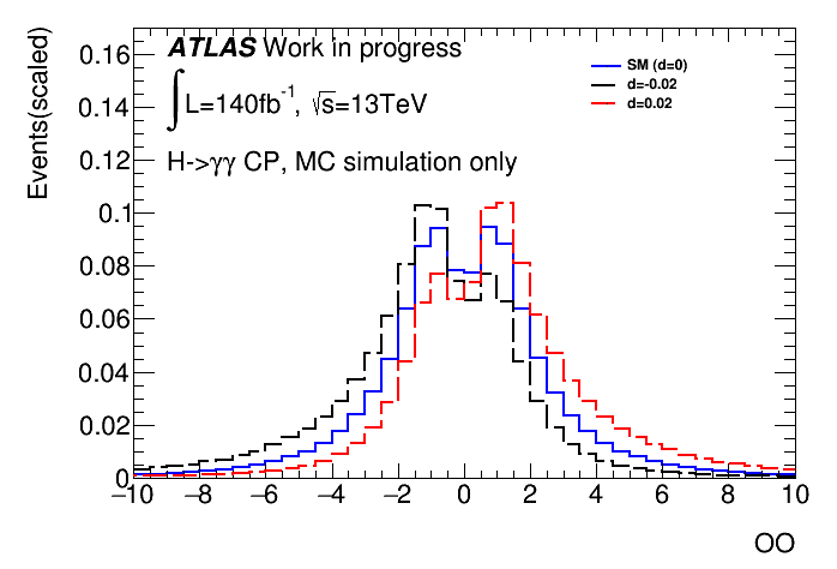
\includegraphics[width=.7\textwidth]{figure/OOind.png}
	\caption{Optimal Observable distribution in VBF process, with $\tilde{d}=-0.02$, $\tilde{d}=0$ (SM) and $\tilde{d}=0.02$}
	\label{fig:OOwithd}
\end{figure}

\paragraph{}The package HAWK[/ref] provides a calculation for VBF and VH process matrix element, with the kinematic variables in final state (4-momenta of the Higgs boson and 2 tagging jets in VBF). For the initial state, the momentum fraction Bjorken $x_1$($x_2$) of parton can be derived by energy-momentum conservation: 

\begin{center}
\begin{math}
x_{1,2}^{reco}=\frac{m_{Hjj}}{\sqrt{s}}e^{\pm y_{Hjj}}
\end{math}
\end{center}

Where $m_{Hjj}$ and $y_{Hjj}$ are the invariant mass and pseudo rapidity of Higgs+2 tagging jets system. The matrix element calculation performs a summation of all possible flavor configurations in initial and final state ij->klH weighted by CT10 leading order parton distribution functions(PDFs.). 

\begin{center}
\begin{math}
2Re(\mathcal{M}^{\ast}_{SM}\mathcal{M}_{CP-odd}) = \sum_{i,j,k,l} f_i(x_1)f_j(x_2)2Re((\mathcal{M}_{SM}^{ij \to klH})^{\ast} \mathcal{M}_{CP-odd}^{ij\to klH} ) 
\end{math}
\\
\begin{math}
|\mathcal{M}_{SM}|^2 = \sum_{i,j,k,l} f_i(x_1)f_j(x_2)|\mathcal{M}_{SM}^{ij \to klH}|^2
\end{math}
\end{center}




